%!Mode:: "TeX:UTF-8"
\documentclass[a4paper,11pt,UTF8]{ctexart}

\usepackage{indentfirst} %缩进
\usepackage{xeCJK}    %使用系统字体
\usepackage{fancyhdr} %自定义页眉页脚
\pagestyle{plain}                   %不设置页眉页脚
\usepackage{amsmath, amsthm, amssymb, amsfonts} %数学公式
\usepackage[a4paper,left=3cm,right=3cm,top=3cm,bottom=3cm]{geometry}
%\usepackage[tmargin=1in,bmargin=1in,lmargin=1.25in,rmargin=1.25in]{geometry}.
\usepackage{booktabs} %插入表格
\usepackage[section]{placeins} %避免浮动
\usepackage{listings} %插入代码
\usepackage{ctex}     %中文宏包
\usepackage{bm}
\usepackage[svgnames, table]{xcolor} %彩色表格
\usepackage{algorithm}          %伪代码
\usepackage{algorithmicx}
\usepackage{algpseudocode}
\usepackage{algorithm,algpseudocode,float}
\usepackage{lipsum}
\usepackage{enumitem}           %调整列举环境
\usepackage{url}
\usepackage{fontspec,xunicode}
\defaultfontfeatures{Mapping=tex-text} %如果没有它,会有一些 tex 特殊字符无法正常使用,比如连字符。

\usepackage{graphicx}
\graphicspath{{imgs/}}

%%%%%%%%%%%%%%%%%%%%%%%%%%%%%%%%%%%%%%%%%%%%%%%%%%%%%%%%%%%%%%%%
% 缩进及行间距
%%%%%%%%%%%%%%%%%%%%%%%%%%%%%%%%%%%%%%%%%%%%%%%%%%%%%%%%%%%%%%%%
\setlength{\parindent}{22pt} %重新定义缩进长度
\setlength{\baselineskip}{20pt}  %定义行间距
%\renewcommand{\baselinestretch}{1.1} %定义行间距

%%%%%%%%%%%%%%%%%%%%%%%%%%%%%%%%%%%%%%%%%%%%%%%%%%%%%%%%%%%%%%%%
% 列表设置
%%%%%%%%%%%%%%%%%%%%%%%%%%%%%%%%%%%%%%%%%%%%%%%%%%%%%%%%%%%%%%%%
\setenumerate{fullwidth,itemindent=\parindent,listparindent=\parindent,itemsep=0ex,partopsep=0pt,parsep=0ex}
\setenumerate[2]{label=\alph*),leftmargin=1.5em}  %二级item设置
\setitemize{itemindent=38pt,leftmargin=0pt,itemsep=-0.4ex,listparindent=26pt,partopsep=0pt,parsep=0.5ex,topsep=-0.25ex}
\setdescription{itemindent=38pt,leftmargin=0pt,itemsep=-0.4ex,listparindent=26pt,partopsep=0pt,parsep=0.5ex,topsep=-0.25ex}

%%%%%%%%%%%%%%%%%%%%%%%%%%%%%%%%%%%%%%%%%%%%%%%%%%%%%%%%%%%%%%%%
% 图的标题行间距设置
%%%%%%%%%%%%%%%%%%%%%%%%%%%%%%%%%%%%%%%%%%%%%%%%%%%%%%%%%%%%%%%%
\newcommand{\bottomcaption}{%
\setlength{\abovecaptionskip}{6pt}%
\setlength{\belowcaptionskip}{6pt}%
\caption}


%%%%%%%%%%%%%%%%%%%%%%%%%%%%%%%%%%%%%%%%%%%%%%%%%%%%%%%%%%%%%%%%
% 字体定义
%%%%%%%%%%%%%%%%%%%%%%%%%%%%%%%%%%%%%%%%%%%%%%%%%%%%%%%%%%%%%%%%
% \setmainfont{Times New Roman}  %默认英文字体.serif是有衬线字体sans serif无衬线字体
\setmonofont{Consolas}
\setCJKmainfont[ItalicFont={楷体}, BoldFont={黑体}]{宋体}%衬线字体 缺省中文字体为
\setCJKsansfont{黑体}
\punctstyle{hangmobanjiao}
%-----------------------xeCJK下设置中文字体------------------------------%
\setCJKfamilyfont{song}{SimSun}                             %宋体 song
\newcommand{\song}{\CJKfamily{song}}
\setCJKfamilyfont{fs}{FangSong}                      %仿宋  fs
\newcommand{\fs}{\CJKfamily{fs}}
\setCJKfamilyfont{ktgb}{KaiTi}                      %楷体2312 ktgb
\newcommand{\ktgb}{\CJKfamily{ktgb}}
\setCJKfamilyfont{yh}{Microsoft YaHei}                    %微软雅黑 yh
\newcommand{\yh}{\CJKfamily{yh}}
\setCJKfamilyfont{hei}{SimHei}                              %黑体  hei
\newcommand{\hei}{\CJKfamily{hei}}
\setCJKfamilyfont{hwxk}{STXingkai}                                %华文行楷  hwxk
\newcommand{\hwxk}{\CJKfamily{hwxk}}
%------------------------------设置字体大小------------------------%
\newcommand{\shiyanbaogao}{\fontsize{36pt}{\baselineskip}\selectfont}
\newcommand{\chuhao}{\fontsize{42pt}{\baselineskip}\selectfont}     %初号
\newcommand{\xiaochuhao}{\fontsize{36pt}{\baselineskip}\selectfont} %小初号
\newcommand{\yihao}{\fontsize{28pt}{\baselineskip}\selectfont}      %一号
\newcommand{\erhao}{\fontsize{21pt}{\baselineskip}\selectfont}      %二号
\newcommand{\xiaoerhao}{\fontsize{18pt}{\baselineskip}\selectfont}  %小二号
\newcommand{\sanhao}{\fontsize{15.75pt}{\baselineskip}\selectfont}  %三号
\newcommand{\sihao}{\fontsize{14pt}{\baselineskip}\selectfont}       %四号
\newcommand{\xiaosihao}{\fontsize{12pt}{\baselineskip}\selectfont}  %小四号
\newcommand{\wuhao}{\fontsize{10.5pt}{\baselineskip}\selectfont}    %五号
\newcommand{\xiaowuhao}{\fontsize{9pt}{\baselineskip}\selectfont}   %小五号
\newcommand{\liuhao}{\fontsize{7.875pt}{\baselineskip}\selectfont}  %六号
\newcommand{\qihao}{\fontsize{5.25pt}{\baselineskip}\selectfont}    %七号

%%%%%%%%%%%%%%%%%%%%%%%%%%%%%%%%%%%%%%%%%%%%%%%%%%%%%%%%%%%%%%%%
% 图题字体大小相同
%%%%%%%%%%%%%%%%%%%%%%%%%%%%%%%%%%%%%%%%%%%%%%%%%%%%%%%%%%%%%%%%
\usepackage{caption}
\captionsetup{font={footnotesize}}   % footnotesize = 9pt
\captionsetup[lstlisting]{font={footnotesize}}

%%%%%%%%%%%%%%%%%%%%%%%%%%%%%%%%%%%%%%%%%%%%%%%%%%%%%%%%%%%%%%%%
% 重定义枚举编号为 1),2)...
%%%%%%%%%%%%%%%%%%%%%%%%%%%%%%%%%%%%%%%%%%%%%%%%%%%%%%%%%%%%%%%%
\renewcommand{\labelenumi}{\theenumi)}


%%%%%%%%%%%%%%%%%%%%%%%%%%%%%%%%%%%%%%%%%%%%%%%%%%%%%%%%%%%%%%%%
% 重定义section标题
%%%%%%%%%%%%%%%%%%%%%%%%%%%%%%%%%%%%%%%%%%%%%%%%%%%%%%%%%%%%%%%%
\CTEXsetup[format={\sihao\CJKfamily{zhhei}\zihao{4}},number={\chinese{section}},name={,、~},aftername={},indent={0pt},beforeskip={6pt},afterskip={6pt},format+={\flushleft}]{section}
\CTEXsetup[format={\Large\bfseries\CJKfamily{zhkai}\zihao{4}},name={(,)},number={\chinese{subsection}},aftername={},indent={22pt},beforeskip={14pt},afterskip={2pt}]{subsection}
\CTEXsetup[number={\chinese{section}},name={附录, ~~ }]{appendix}



%%%%%%%%%%%%%%%%%%%%%%%%%%%%%%%%%%%%%%%%%%%%%%%%%%%%%%%%%%%%%%%%
% 标题名称中文化
%%%%%%%%%%%%%%%%%%%%%%%%%%%%%%%%%%%%%%%%%%%%%%%%%%%%%%%%%%%%%%%%
\renewcommand\figurename{\hei 图}
\renewcommand\tablename{\hei 表}
\renewcommand\lstlistingname{\hei 代码}
\renewcommand{\algorithmicrequire}{\textbf{输入:}}
\renewcommand{\algorithmicensure}{\textbf{输出:}}
\newtheorem{define}{定义}

%%%%%%%%%%%%%%%%%%%%%%%%%%%%%%%%%%%%%%%%%%%%%%%%%%%%%%%%%%%%%%%%
% 代码设置
%%%%%%%%%%%%%%%%%%%%%%%%%%%%%%%%%%%%%%%%%%%%%%%%%%%%%%%%%%%%%%%%
\lstset{
 columns=fixed,
 numbers=left,                                        % 在左侧显示行号
 numberstyle=\tiny\color{gray},                       % 设定行号格式
 frame=single,                                        % 单线背景边框
 breaklines=true,                                     % 设定LaTeX对过长的代码行进行自动换行
 keywordstyle=\color[RGB]{40,40,255},                 % 设定关键字颜色
 numberstyle=\footnotesize\color{darkgray},
 commentstyle=\it\color[RGB]{0,96,96},                % 设置代码注释的格式
 stringstyle=\rmfamily\slshape\color[RGB]{128,0,0},   % 设置字符串格式
 showstringspaces=false,                              % 不显示字符串中的空格
 language=java,                                        % 设置语言
 basicstyle=\linespread{1.0}\xiaowuhao\ttfamily,                      % 字体字号
 %lineskip=10pt,
 %baselinestretch=1,
}

%%%%%%%%%%%%%%%%%%%%%%%%%%%%%%%%%%%%%%%%%%%%%%%%%%%%%%%%%%%%%%%%
% 伪代码分页
%%%%%%%%%%%%%%%%%%%%%%%%%%%%%%%%%%%%%%%%%%%%%%%%%%%%%%%%%%%%%%%%
\makeatletter
\renewcommand{\ALG@name}{算法}
\newenvironment{breakablealgorithm}
  {% \begin{breakablealgorithm}
   \begin{center}
     \refstepcounter{algorithm}% New algorithm
     \hrule height.8pt depth0pt \kern2pt% \@fs@pre for \@fs@ruled
     \renewcommand{\caption}[2][\relax]{% Make a new \caption
       {\raggedright\textbf{\ALG@name~\thealgorithm} ##2\par}%
       \ifx\relax##1\relax % #1 is \relax
         \addcontentsline{loa}{algorithm}{\protect\numberline{\thealgorithm}##2}%
       \else % #1 is not \relax
         \addcontentsline{loa}{algorithm}{\protect\numberline{\thealgorithm}##1}%
       \fi
       \kern2pt\hrule\kern2pt
     }
  }{% \end{breakablealgorithm}
     \kern2pt\hrule\relax% \@fs@post for \@fs@ruled
   \end{center}
  }
\makeatother



\begin{document}
\xiaosihao\song

\begin{titlepage}
\center{\yihao{\hei{机器学习课程实验报告}}}
\vspace{6cm}
\center{\erhao{\ktgb{多项式拟合正弦曲线}}}
\vspace{4cm}

\begin{center}
\begin{large}
\begin{tabular}{rc}
\xiaoerhao{\hei{学\qquad 号}}& \hspace{1.7cm}\xiaoerhao{\hei{1180301007\hspace{1.7cm}}} \\
\cline{2-2}\\
\xiaoerhao{\hei{姓\qquad 名}}& \xiaoerhao{\hei{赵锦涛}}\\
\cline{2-2}\\
\xiaoerhao{\hei{实验时间}}& \xiaoerhao{\hei{2020年9月}}\\
\cline{2-2}
\end{tabular}
\end{large}
\end{center}
\vfill \hfill
\end{titlepage}
\clearpage


\setlength{\parskip}{6pt}  %定义段间距

\section{实验目的:}
掌握最小二乘法求解(无惩罚项的损失函数)、掌握加惩罚项(2范数)的损失函数优化、梯度下降法、共轭梯度法、理解过拟合、克服过拟合的方法(如加惩罚项、增加样本)。
\section{实验要求:}
\begin{enumerate}
	\item 生成数据,加入噪声;
	\item 用高阶多项式函数拟合曲线;
	\item 用解析解求解两种loss的最优解(无正则项和有正则项);
	\item 优化方法求解最优解(梯度下降,共轭梯度);
	\item 用你得到的实验数据,解释过拟合;
	\item 用不同数据量,不同超参数,不同的多项式阶数,比较实验效果;
	\item 语言不限,可以用matlab,python。求解解析解时可以利用现成的矩阵求逆。梯度下降,共轭梯度要求自己求梯度,迭代优化自己写。不许用现成的平台,例如pytorch,tensorflow的自动微分工具。	
\end{enumerate}
\section{实验环境:}

Python 3.8, Windows 10

\section{实验原理:}
\subsection{数据生成}
训练数据通过Python Numpy库在指定区间内均匀选定n个x坐标点(数据点的数目可指定),然后调用Numpy库中的sin函数计算对应$sin(2\pi x)$的y坐标值,接着调用Python Random库的gauss函数为数据加入噪声,其中高斯分布的均值设为0,标准差设为0.016。图1为在[0,1]区间上生成的40个数据点:
\begin{figure}[htbp]
	\centering
	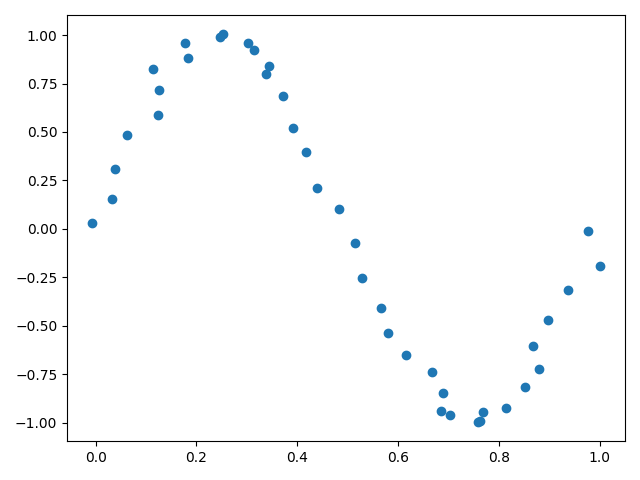
\includegraphics[width=0.6\textwidth]{datademo.png}
	\bottomcaption{生成数据点示例}
\end{figure}

\subsection{最小二乘法求解}
给定n个正弦数据点$[(x_{1},y_{1}), (x_{2}, y_{2}),...,(x_{n}, y_{n})]$,使用形如$y(x, w)=w_{0}+w_{1} x+\cdots+w_{m} x^{m}=\sum_{i=0}^{m} w_{i} x^{i}$的多项式拟合曲线,记
$\bm{x_{i}} = [1, x, x^{2}, ..., x^{m}]^{T}$,$\bm{y} = [y_{1}, y_{2},..., y_{n}]^{T}$,$\bm{w} = [w_{0}, w_{2},..., w_{m}]^{T}$,$\bm{A} = [\bm{x_{1}}^{T}, \bm{x_{2}}^{T},...,\bm{x_{n}}^{T}]^{T}$。建立误差函数$$E(\bm{w}) = \frac{1}{2}(\bm{Aw} - \bm{y}) ^{T}(\bm{Aw} - \bm{y})$$ \\
1. 无正则项 \\
求导得,$$\frac{\partial E(\bm{w})}{\partial \bm{w}} = \bm{A}^{T}\bm{Aw} - \bm{A}^{T}\bm{y}$$
令导数为0,有
$$ \bm{A}^{T}\bm{Aw} = \bm{A}^{T}\bm{y}$$
若$\bm{A}$列满秩,有$$\bm{w} = (\bm{A}^{T}\bm{A})^{-1}\bm{A}^{T}\bm{y}$$
2. 有正则项 \\
加入正则项,误差函数变为
$$E(\bm{w}) = \frac{1}{2}[(\bm{Aw} - \bm{y}) ^{T}(\bm{Aw} - \bm{y}) + \lambda\bm{w}^{T}\bm{w}] $$
求导得,$$\frac{\partial E(\bm{w})}{\partial \bm{w}} = \bm{A}^{T}\bm{Aw} - \bm{A}^{T}\bm{y} + \lambda \bm{w}$$
令导数为0,同理可解得
$$\bm{w} = (\bm{A}^{T}\bm{A} + \lambda\bm{E})^{-1}\bm{A}^{T}\bm{y}$$

\subsection{梯度下降法}
梯度的方向是函数增长最快的方向,已知误差函数$E(\bm{w}) = \frac{1}{2}(\bm{Aw} - \bm{y}) ^{T}(\bm{Aw} - \bm{y})$,可以通过梯度下降的方法来迭代求得最小误差以及对应的参数值。\\
对于$\bm{w}$向量,其梯度表达式为$$ \frac{\partial E(\bm{w})}{\partial \bm{w}} = \bm{A}^{T}\bm{Aw} - \bm{A}^{T}\bm{y} $$
设学习率为$\alpha$,则可以用当前$\bm{w}$减去当前的梯度来更新$\bm{w}$的值,迭代该过程,从而不断逼近使误差函数取最小时的$\bm{w}$。迭代计算公式为$$ \bm{w}_{i+1} = \bm{w}_{i} - \alpha \bm{A}^{T}(\bm{A}\bm{w}_{i} - \bm{y}) $$
加入正则项后(误差函数与解析法有正则项时相同),同理可得迭代计算公式
$$\bm{w}_{i+1} = (1 - \lambda \alpha)\bm{w}_{i} - \alpha \bm{A}^{T}(\bm{A}\bm{w}_{i} - \bm{y}) $$

\subsection{共轭梯度}
二次型,是关于向量的二次数值型函数,形如: $$ f(\bm{x}) = \frac{1}{2} \bm{x}^{T}\bm{Ax} - \bm{b}^{T}\bm{x} + c$$
由线性代数知识可得,当$\bm{A}$为对称正定阵时,$f(\bm{x})$的最小值由$\bm{Ax} = \bm{b}$的解给出。由上文讨论可得到,误差函数为
\begin{equation}	
	\begin{aligned}
		E(\bm{w}) &= \frac{1}{2}(\bm{Aw} - \bm{y}) ^{T}(\bm{Aw} - \bm{y}) \\
 		&= \frac{1}{2}(\bm{w}^{T}\bm{A}^{T}\bm{Aw} - 2\bm{y}^{T}\bm{Aw} + \bm{y}^{T}\bm{y}) \nonumber
	\end{aligned}
\end{equation}
令$\bm{A'} = \bm{A}^{T}\bm{A}, \bm{b} = \bm{A}^{T}\bm{y}, c = \bm{y}^{T}\bm{y},$误差函数可化为二次型
$$ E(\bm{w}) = \frac{1}{2}\bm{w}^{T}\bm{A'}\bm{w} - \bm{b}^{T}\bm{w} + c$$
所以求误差函数最小可以通过求$\bm{A'w} = \bm{b}$的解得出。 \\
\indent 最速下降法在收敛中其早期的迭代步骤往往在沿着同一个方向,而共轭梯度法的思想是选择一系列正交的搜索方向$\bm{d_{0}}, ... \bm{d_{n-1}}$,
在每个方向上移动适当距离,使得刚好消除误差向量在该方向上的分量,当迭代结束后,会移动到最小值点。在这里引入残差向量的概念
$$ \bm{r_{i}} = \bm{b} - \bm{A}\bm{x}_{i}$$
由线性代数知识,可给出共轭梯度法计算过程:
\begin{equation}
\nonumber
\begin{split} 
\bm{d_{0}} &= \bm{r_{0}} = \bm{b_{0}} - \textbf{A} \bm{x_{0}} \\ 
\alpha_{i} &= \frac{\bm{r_{i}}^T \bm{r_{i}}} {\bm{d_{i}}^T \textbf{A} \bm{d_{i}}} \qquad  \\
\bm{x_{i+1}} &= \bm{x_{i}} + \alpha_{i} \bm{d_{i}} \\ 
\bm{r_{i+1}} &= \bm{r_{i}} - \alpha_{i} \textbf{A} \bm{d_{i}} \\ 
\beta_{i+1} &= \frac{\bm{r_{i+1}}^T \bm{r_{i+1}}} {\bm{r_{i}}^T \bm{r_{i}}} \\ 
\bm{d_{i+1}} &= \bm{r_{i+1}} + \beta_{i+1} \bm{d_{i}} 
\end{split}
\end{equation}
\section{实验结果与分析}

\subsection{最小二乘法求解}
如图2,当阶数为10,数据点个数为11时,出现过拟合现象。
\begin{figure}[htbp]
	\centering
	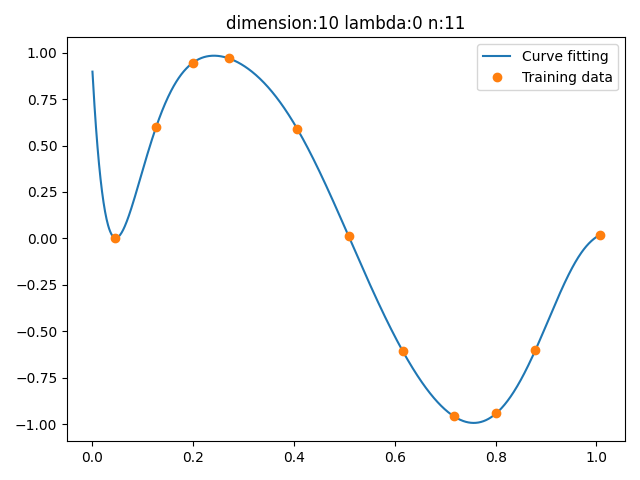
\includegraphics[width=0.6\textwidth]{1_1.png}
	\bottomcaption{最小二乘法求解一}
\end{figure}
为解决过拟合现象,可加入正则项,令$lambda = 0.001$,如图3。
\begin{figure}[H]
\centering %图片全局居中
%并排几个图,就要写几个minipage
\begin{minipage}[b]{0.45\textwidth} %所有minipage宽度之和要小于1,否则会自动变成竖排
\centering %图片局部居中
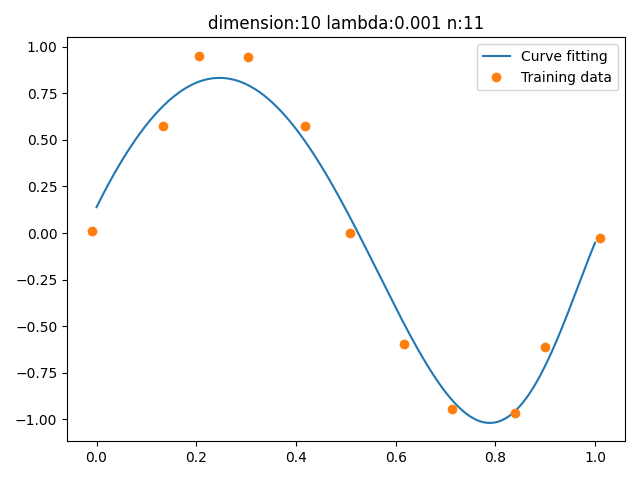
\includegraphics[width=1\textwidth]{1_2.png} %此时的图片宽度比例是相对于这个minipage的,不是全局
\caption{最小二乘法求解二}
\end{minipage}
\begin{minipage}[b]{0.45\textwidth} %所有minipage宽度之和要小于1,否则会自动变成竖排
\centering %图片局部居中
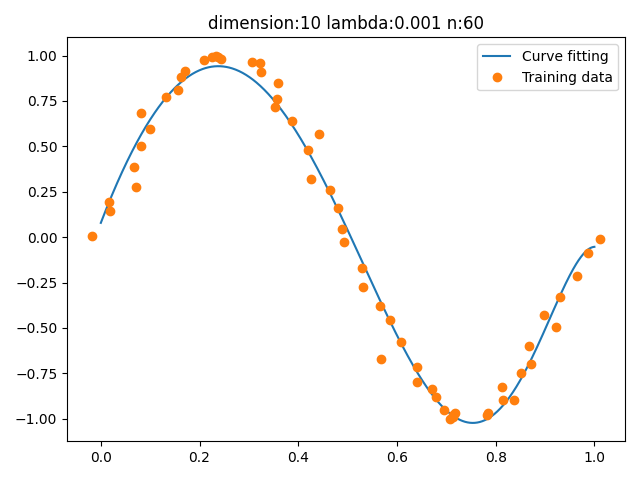
\includegraphics[width=1\textwidth]{1_3.png}%此时的图片宽度比例是相对于这个minipage的,不是全局
\caption{最小二乘法求解三}
\end{minipage}
\end{figure}
也可增加数据点数量以解决过拟合现象,令$n=60$,如图4。
\subsection{梯度下降法}
当阶数为10,数据点个数为11时,令正则项系数$lambda = 0$,观察图像右端出现过拟合现象,令$lambda$分别为0.001和0.005,对比可发现正则项系数的增大一定程度上抑制了过拟合现象,但也对模型产生了负面影响。
\begin{figure}[htbp]
	\centering
	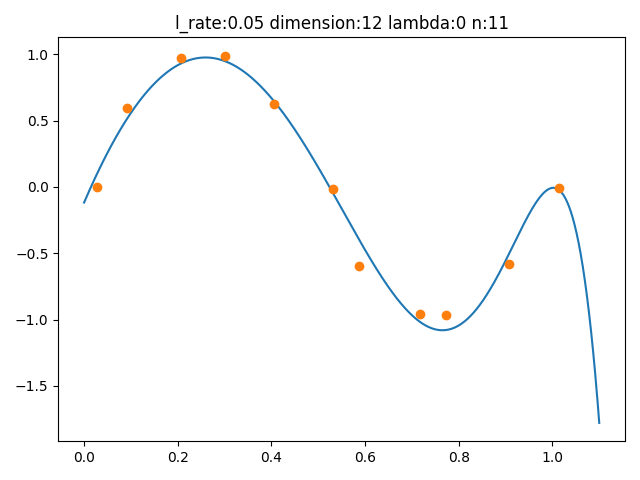
\includegraphics[width=0.45\textwidth]{2_1.png}
	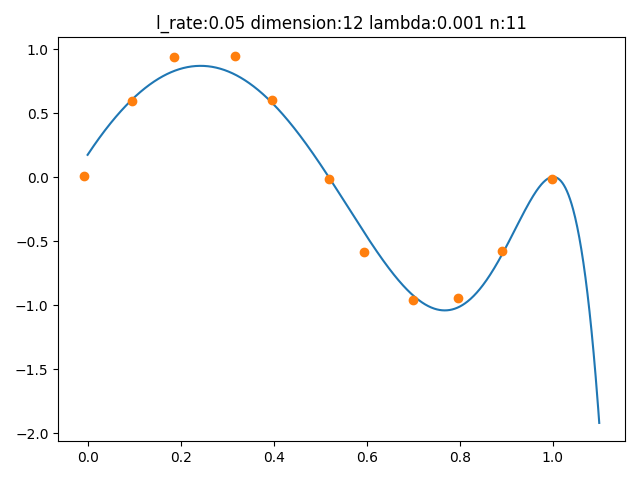
\includegraphics[width=0.45\textwidth]{2_2.png}
	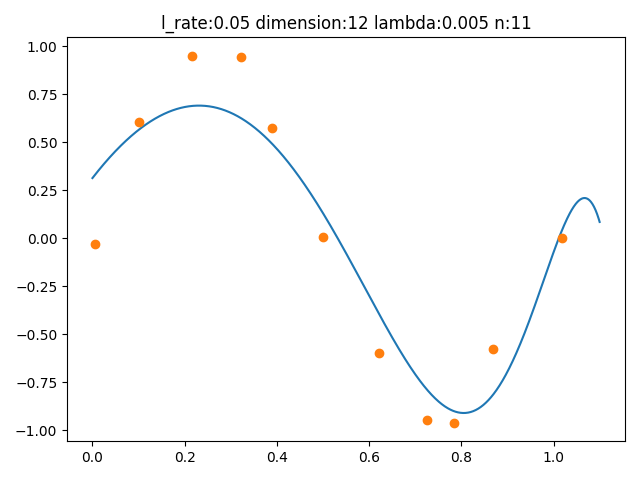
\includegraphics[width=0.5\textwidth]{2_3.png}
	\bottomcaption{梯度下降}
\end{figure}
当增加样本点使$n = 60$后,可发现训练效果较好,也未出现显著的过拟合现象。
\begin{figure}[htbp]
	\centering
	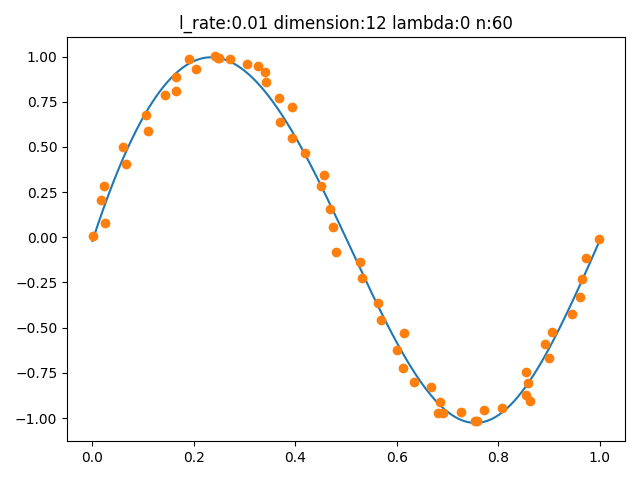
\includegraphics[width=0.6\textwidth]{2_4.png}
	\bottomcaption{梯度下降法,$n=60$}
\end{figure}
在实验中还发现,相较于最小二乘求解方法,梯度下降法训练时间一般较长,收敛速度较慢。对于阶数为12,数据点数为60的数据,最小二乘方法所需时间为0.1698秒,而学习率为0.05的梯度下降法训练同样的数据所需时间为103.4624秒。


\subsection{共轭梯度法}
如图7,为使用共轭梯度法拟合曲线效果,阶数为12,数据点个数为60,迭代次数也为60。从图中可以看出拟合效果较好,未出现过拟合现象。除此之外,运行时间较短,仅为0.1317秒
\begin{figure}[htbp]
	\centering
	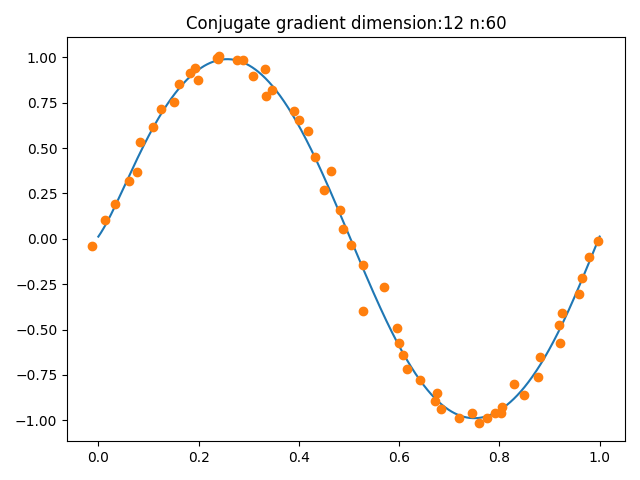
\includegraphics[width=0.6\textwidth]{3_1.png}
	\bottomcaption{共轭梯度法}
\end{figure}

\subsection{总结}
从实验结果中可以得到,数据点越多,训练得到的模型拟合效果越好。其次,模型的复杂度与参数个数有关,模型参数越多,也即设置的多项式阶数越高,其拟合能力越强。当参数过多时,会出现过拟合现象,每个数据点都落在拟合曲线上,但此时拟合出的曲线离正弦曲线相差较远,此时可以通过加入正则项或者叫做惩罚项来调整模型的复杂度以降低过拟合现象,或者增多样本数据,避免数据过少导致的特殊曲线情况。 \par
加入正则项后,正则项的系数会影响模型训练的好坏。当正则项系数设置过小时,难抑制过拟合现象。当正则项系数设置过大时,模型复杂度主要与参数有关,数据对模型的影响比较小,导致学习能力较差,会出现欠拟合现象。需要正确设置正则项系数,才能获得较好的模型训练效果。 \par
在梯度下降中,需要设置学习率,当学习率设置的过小时,收敛过程将变得十分缓慢。而当学习率设置的过大时,梯度可能会在最小值附近来回振荡,甚至可能无法收敛。所以需要合理设置学习率,根据相关文献资料,可以使学习率服从指数衰减,这样可以加快收敛速度,同时避免在极值点附近出现过分振荡。共轭梯度法对比梯度下降法,其收敛速度较快。原因是使用了相互正交的搜索向量,迭代次数更少,收敛速度更快。

\section{代码实现:}

本次实验共有7个文件,其名称和作用分别为:
\begin{itemize}
	\item \emph{datagen.py} \quad 生成训练数据
	\item \emph{curveplot.py} \quad 绘制拟合曲线
	\item \emph{loss.py} \quad 计算损失函数
	\item \emph{linear\_regression.py} \quad 最小二乘法拟合曲线
	\item \emph{gradient.py} \quad 梯度下降法拟合曲线
	\item \emph{gradient\_gpu.py} \quad 使用Cupy库的梯度下降法拟合曲线,可使用CUDA进行GPU矩阵运算
	\item \emph{conjugate\_gradient.py} \quad 共轭梯度法拟合曲线
\end{itemize}
\par
实现细节请见具体代码文件。	

\begin{thebibliography}{99} 
\bibitem{ref1}断鸿声里,立尽斜阳.共轭梯度法通俗讲义 | 断鸿声里,立尽斜阳[EB/OL].https://flat2010.github.io/2018/10/26/共轭梯度法通俗讲义/\#8-共轭梯度法,2018-10-25.
\bibitem{ref2}刘建平Pinard.梯度下降(Gradient Descent)小结[EB/OL].https://www.cnblogs.com/pinard/p/5970503.html,2016-10-17.
\bibitem{ref3}LLLiuye.学习率(Learning rate)的理解以及如何调整学习率[EB/OL].https://www.cnblogs.com/lliuye/p/9471231.html,2018-08-13.
\end{thebibliography}

% \begin{lstlisting}[caption={一段C代码},captionpos=b]
% #include <stdio.h>
% int main (int argc, char *argv[]){
%   printf("Hello world!");
% }
% \end{lstlisting}


\end{document}
